\documentclass[landscape,final,a0paper,fontscale=0.285]{baposter}

\usepackage{calc}
\usepackage{graphicx}
\usepackage{amsmath}
\usepackage{amssymb}
\usepackage{relsize}
\usepackage{multirow}
\usepackage{rotating}
\usepackage{bm}
\usepackage{url}

\usepackage{graphicx,subfigure}
\usepackage{multicol}

%\usepackage{times}
%\usepackage{helvet}
%\usepackage{bookman}
\usepackage{palatino}

\newcommand{\captionfont}{\footnotesize}

\graphicspath{{images/}{../images/}}
\usetikzlibrary{calc}

\newcommand{\SET}[1]  {\ensuremath{\mathcal{#1}}}
\newcommand{\MAT}[1]  {\ensuremath{\boldsymbol{#1}}}
\newcommand{\VEC}[1]  {\ensuremath{\boldsymbol{#1}}}
\newcommand{\Video}{\SET{V}}
\newcommand{\video}{\VEC{f}}
\newcommand{\track}{x}
\newcommand{\Track}{\SET T}
\newcommand{\LMs}{\SET L}
\newcommand{\lm}{l}
\newcommand{\PosE}{\SET P}
\newcommand{\posE}{\VEC p}
\newcommand{\negE}{\VEC n}
\newcommand{\NegE}{\SET N}
\newcommand{\Occluded}{\SET O}
\newcommand{\occluded}{o}

%%%%%%%%%%%%%%%%%%%%%%%%%%%%%%%%%%%%%%%%%%%%%%%%%%%%%%%%%%%%%%%%%%%%%%%%%%%%%%%%
%%%% Some math symbols used in the text
%%%%%%%%%%%%%%%%%%%%%%%%%%%%%%%%%%%%%%%%%%%%%%%%%%%%%%%%%%%%%%%%%%%%%%%%%%%%%%%%

%%%%%%%%%%%%%%%%%%%%%%%%%%%%%%%%%%%%%%%%%%%%%%%%%%%%%%%%%%%%%%%%%%%%%%%%%%%%%%%%
% Multicol Settings
%%%%%%%%%%%%%%%%%%%%%%%%%%%%%%%%%%%%%%%%%%%%%%%%%%%%%%%%%%%%%%%%%%%%%%%%%%%%%%%%
\setlength{\columnsep}{1.5em}
\setlength{\columnseprule}{0mm}

%%%%%%%%%%%%%%%%%%%%%%%%%%%%%%%%%%%%%%%%%%%%%%%%%%%%%%%%%%%%%%%%%%%%%%%%%%%%%%%%
% Save space in lists. Use this after the opening of the list
%%%%%%%%%%%%%%%%%%%%%%%%%%%%%%%%%%%%%%%%%%%%%%%%%%%%%%%%%%%%%%%%%%%%%%%%%%%%%%%%
\newcommand{\compresslist}{%
\setlength{\itemsep}{1pt}%
\setlength{\parskip}{0pt}%
\setlength{\parsep}{0pt}%
}

%%%%%%%%%%%%%%%%%%%%%%%%%%%%%%%%%%%%%%%%%%%%%%%%%%%%%%%%%%%%%%%%%%%%%%%%%%%%%%
%%% Begin of Document
%%%%%%%%%%%%%%%%%%%%%%%%%%%%%%%%%%%%%%%%%%%%%%%%%%%%%%%%%%%%%%%%%%%%%%%%%%%%%%

\begin{document}

%%%%%%%%%%%%%%%%%%%%%%%%%%%%%%%%%%%%%%%%%%%%%%%%%%%%%%%%%%%%%%%%%%%%%%%%%%%%%%
%%% Here starts the poster
%%%---------------------------------------------------------------------------
%%%%%%%%%%%%%%%%%%%%%%%%%%%%%%%%%%%%%%%%%%%%%%%%%%%%%%%%%%%%%%%%%%%%%%%%%%%%%%
% Define some colors

%\definecolor{lightblue}{cmyk}{0.83,0.24,0,0.12}
\definecolor{lightblue}{rgb}{0.466,0.145,0.766}

% Draw a video
\newlength{\FSZ}
\newcommand{\drawvideo}[3]{% [0 0.25 0.5 0.75 1 1.25 1.5]
   \noindent\pgfmathsetlength{\FSZ}{\linewidth/#2}
   \begin{tikzpicture}[outer sep=0pt,inner sep=0pt,x=\FSZ,y=\FSZ]
   \draw[color=lightblue!50!black] (0,0) node[outer sep=0pt,inner sep=0pt,text width=\linewidth,minimum height=0] (video) {\noindent#3};
   \path [fill=lightblue!50!black,line width=0pt] 
     (video.north west) rectangle ([yshift=\FSZ] video.north east) 
    \foreach \x in {1,2,...,#2} {
      {[rounded corners=0.6] ($(video.north west)+(-0.7,0.8)+(\x,0)$) rectangle +(0.4,-0.6)}
    }
;
   \path [fill=lightblue!50!black,line width=0pt] 
     ([yshift=-1\FSZ] video.south west) rectangle (video.south east) 
    \foreach \x in {1,2,...,#2} {
      {[rounded corners=0.6] ($(video.south west)+(-0.7,-0.2)+(\x,0)$) rectangle +(0.4,-0.6)}
    }
;
   \foreach \x in {1,...,#1} {
     \draw[color=lightblue!50!black] ([xshift=\x\linewidth/#1] video.north west) -- ([xshift=\x\linewidth/#1] video.south west);
   }
   \foreach \x in {0,#1} {
     \draw[color=lightblue!50!black] ([xshift=\x\linewidth/#1,yshift=1\FSZ] video.north west) -- ([xshift=\x\linewidth/#1,yshift=-1\FSZ] video.south west);
   }
   \end{tikzpicture}
}

\hyphenation{resolution occlusions}
%%
\begin{poster}%
  % Poster Options
  {
  % Show grid to help with alignment
  grid=false,
  % Column spacing
  colspacing=1em,
  % Color style
  bgColorOne=white,
  bgColorTwo=white,
  borderColor=lightblue,
  headerColorOne=black,
  headerColorTwo=lightblue,
  headerFontColor=white,
  boxColorOne=white,
  boxColorTwo=lightblue,
  % Format of textbox
  textborder=roundedleft,
  % Format of text header
  eyecatcher=true,
  headerborder=closed,
  headerheight=0.1\textheight,
%  textfont=\sc, An example of changing the text font
  headershape=roundedright,
  headershade=shadelr,
  headerfont=\Large\bf\textsc, %Sans Serif
  textfont={\setlength{\parindent}{1.5em}},
  boxshade=plain,
%  background=shade-tb,
  background=plain,
  linewidth=2pt
  }
  % Eye Catcher
  {
\includegraphics[height=5em]{images/rent-hop.png}} 
  % Title
  {\bf\text{Evaluation of Customer Interest-Level of Rental Listings}\vspace{0.5em}}
  % Authors
  {\text{ Xialiang Liu, Yihui Wu | NYU CIMS }}
  % University logo
  {% The makebox allows the title to flow into the logo, this is a hack because of the L shaped logo.
    
\includegraphics[height=9.0em]{images/NYU.pdf}
  }

%%%%%%%%%%%%%%%%%%%%%%%%%%%%%%%%%%%%%%%%%%%%%%%%%%%%%%%%%%%%%%%%%%%%%%%%%%%%%%
%%% Now define the boxes that make up the poster
%%%---------------------------------------------------------------------------
%%% Each box has a name and can be placed absolutely or relatively.
%%% The only inconvenience is that you can only specify a relative position 
%%% towards an already declared box. So if you have a box attached to the 
%%% bottom, one to the top and a third one which should be in between, you 
%%% have to specify the top and bottom boxes before you specify the middle 
%%% box.
%%%%%%%%%%%%%%%%%%%%%%%%%%%%%%%%%%%%%%%%%%%%%%%%%%%%%%%%%%%%%%%%%%%%%%%%%%%%%%
    %
    % A coloured circle useful as a bullet with an adjustably strong filling
    \newcommand{\colouredcircle}{%
      \tikz{\useasboundingbox (-0.2em,-0.32em) rectangle(0.2em,0.32em); \draw[draw=black,fill=lightblue,line width=0.03em] (0,0) circle(0.18em);}}

%%%%%%%%%%%%%%%%%%%%%%%%%%%%%%%%%%%%%%%%%%%%%%%%%%%%%%%%%%%%%%%%%%%%%%%%%%%%%%
\headerbox{Contributions}
  {name=intro,column=0,row=0}{
%%%%%%%%%%%%%%%%%%%%%%%%%%%%%%%%%%%%%%%%%%%%%%%%%%%%%%%%%%%%%%%%%%%%%%%%%%%%%%
   In this project, we build a predictive model of how popular an apartment rental listing is associated with the listing content. Good assessment of such listings will allow owners and agents to better understand renters' needs and preferences, and in verse make it easier for renters to find comfortable apartments. 
   \vspace{0.2em}
   
   Dealing with this noisy dataset with expected outliers, we have investigated on tree ensemble methods, \textit{Random Forest} and \textit{Boosted Trees}, to improve our learning model from traditional algorithms of multiclass classification. 
   \vspace{0.2em}
   
   Efforts on feature selection and data cleaning for vocabular features play an important role in interpreting the factors appealing to customers. 
   \vspace{0.3em}
}

%%%%%%%%%%%%%%%%%%%%%%%%%%%%%%%%%%%%%%%%%%%%%%%%%%%%%%%%%%%%%%%%%%%%%%%%%%%%%%
\headerbox{Problem Settings}
  {name=data,column=0,below=intro}{%,bottomaligned=speed
%%%%%%%%%%%%%%%%%%%%%%%%%%%%%%%%%%%%%%%%%%%%%%%%%%%%%%%%%%%%%%%%%%%%%%%%%%%%%%
  This dataset from RentHop (\textit{www.renthop.com}) contains 49352 listings of apartments in New York City. Our objective is to give an estimation based on the available information on the rental listing websites, of the number of inquiries a listing has in the duration that the listing was available on the site, and label it with 3 categories, ``high'', ``medium'', and ``low''. %\vspace{0.3em}
  The data involves multiple features ranging from numbers, dates, categorical features, text, geographical data, and the links of photos. We are aiming at predict the interest-level with this dataset and figure out what are the renter's main considerations.
  With progress of training our learning models, we want to improve the probability of predicting the correct class and the accuracy of prediction. 
  
  {\centering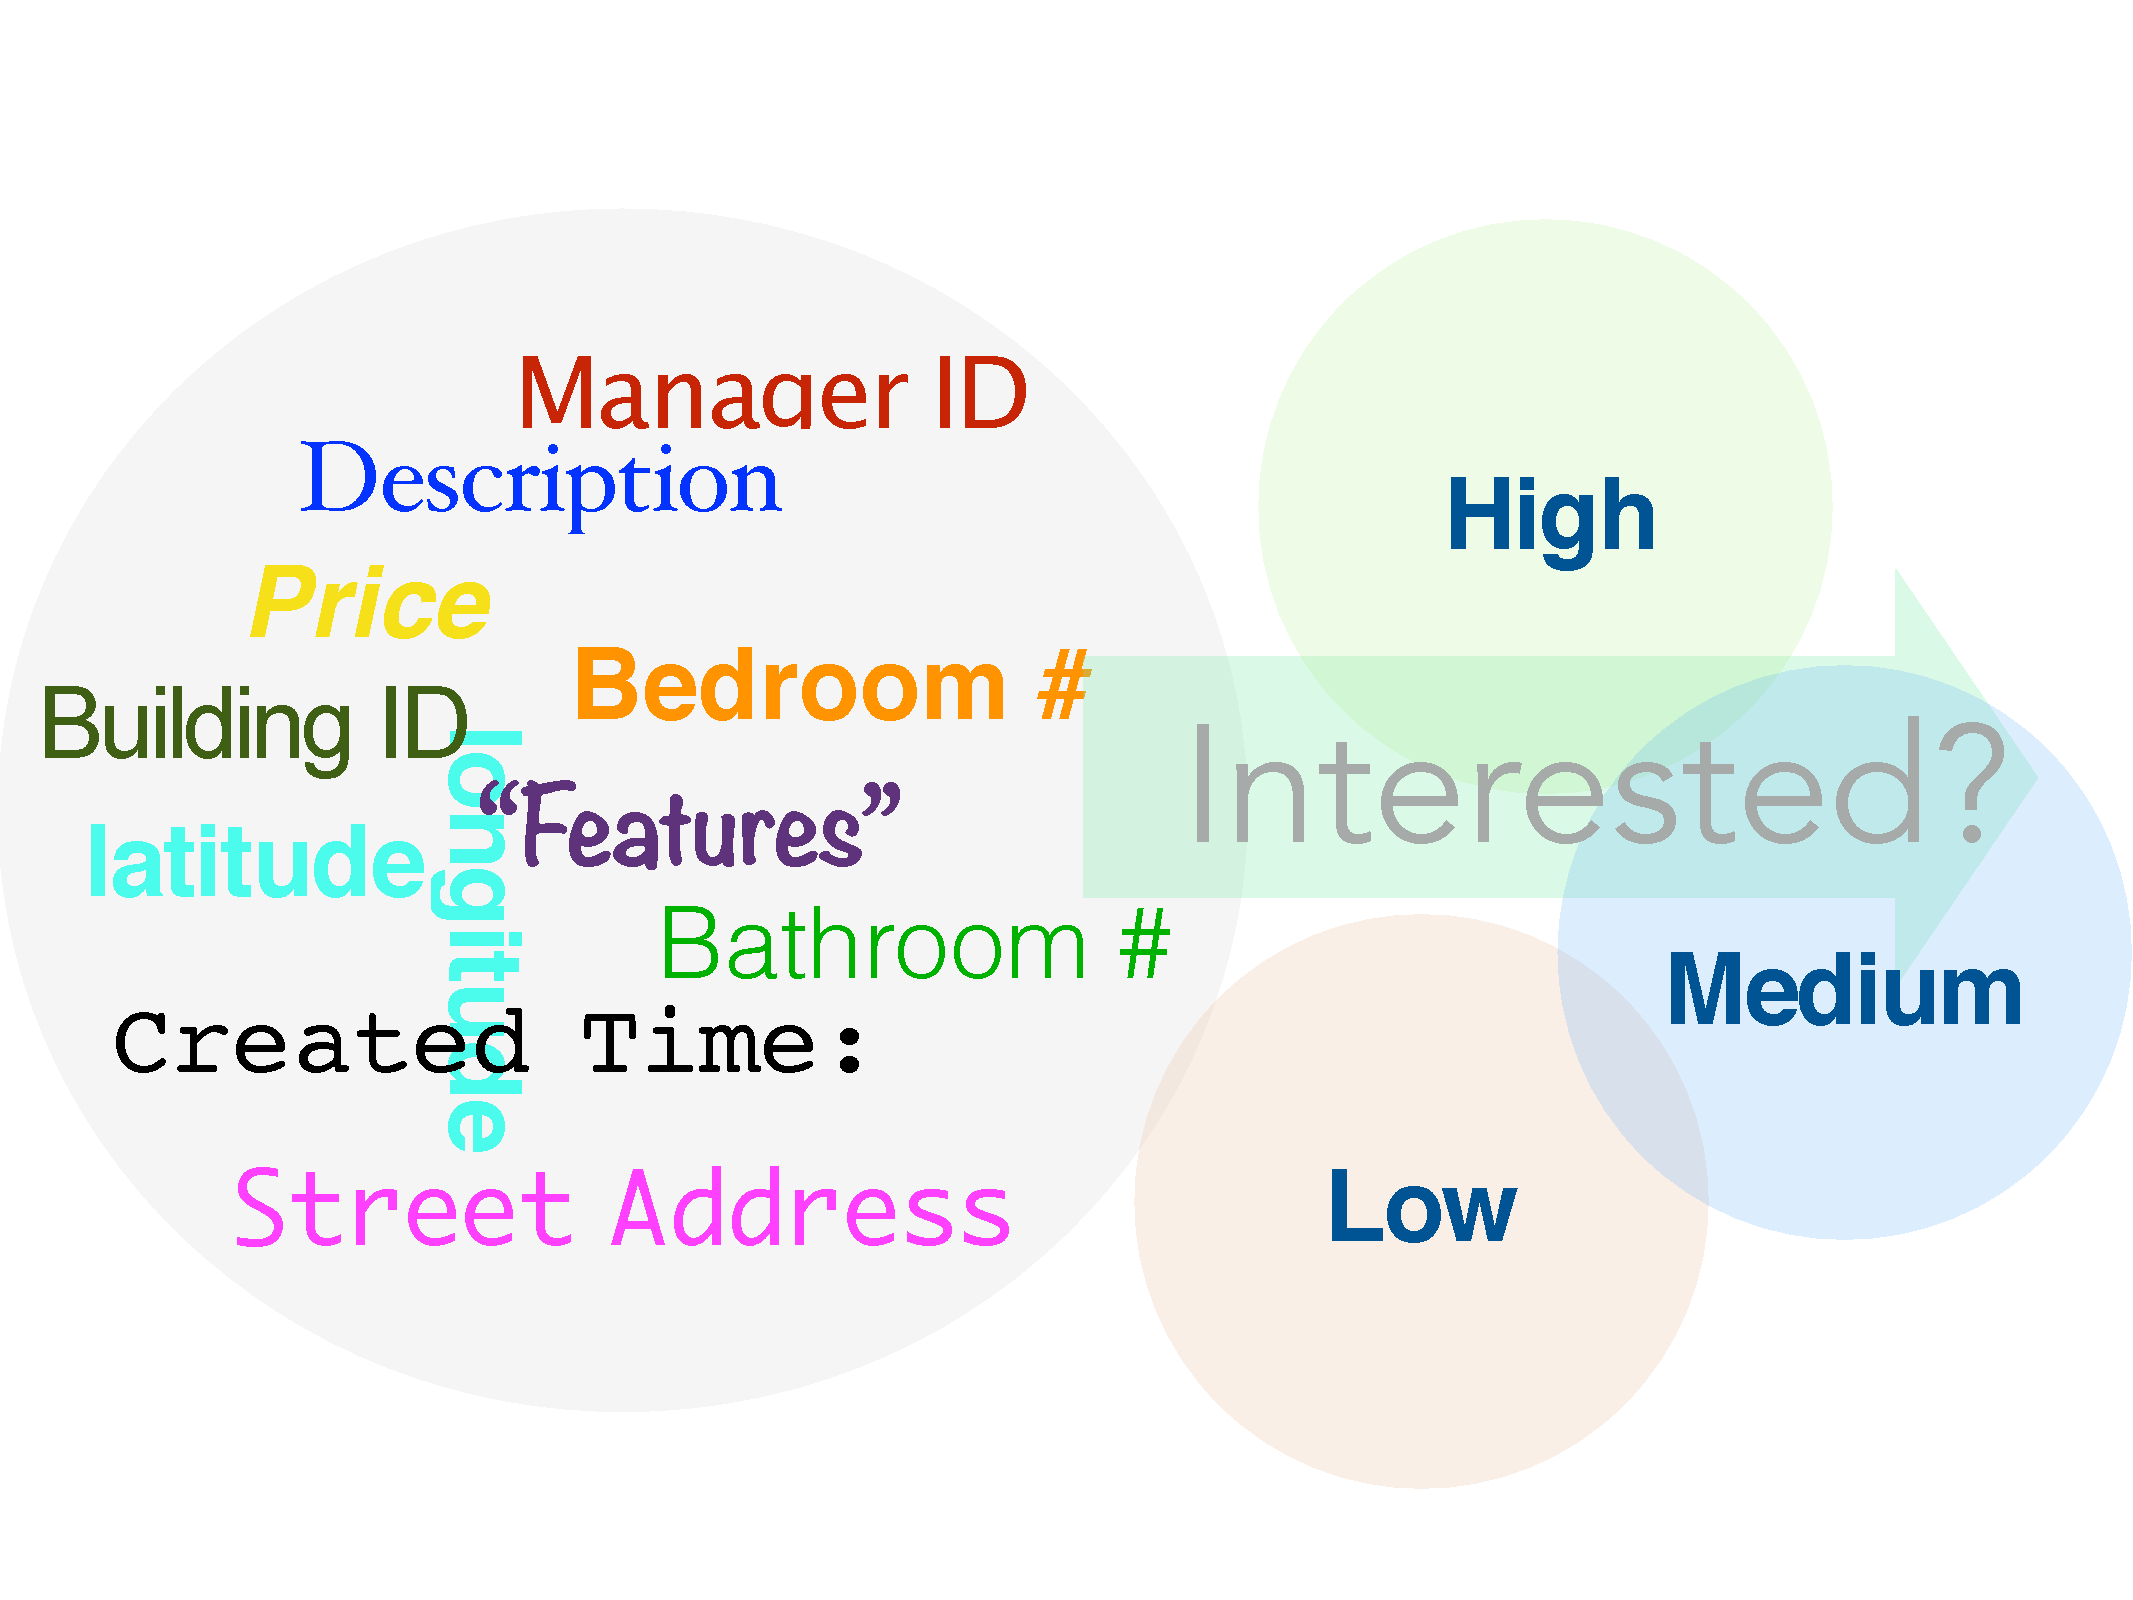
\includegraphics[width=0.9\linewidth]{images/overview.pdf}\\}
  
}

%%%%%%%%%%%%%%%%%%%%%%%%%%%%%%%%%%%%%%%%%%%%%%%%%%%%%%%%%%%%%%%%%%%%%%%%%%%%%%
\headerbox{Features}
  {name=features,column=1,span=2, row=0}{
%%%%%%%%%%%%%%%%%%%%%%%%%%%%%%%%%%%%%%%%%%%%%%%%%%%%%%%%%%%%%%%%%%%%%%%%%%%%%%
  \begin{multicols}{2}
  With access to only five numerical features in the original dataset (number of bedrooms/bathrooms, price, latitude and longitude), we have extracted the following features to improve our learning model.
  \vspace{0.5em}
  
  \noindent\textbf{1. Adding Numerical Features}\vspace{0.2em}
  
  A natural candidate of adding new numerical features is to describe the amount of information. Together with ``created time'' of the listings, we can extract 6 features:\\
  \indent\textbullet ~Number of photos (1)\\
  \indent\textbullet ~Number of features (1)\\
  \indent\textbullet ~Number of description words (1)\\
  \indent\textbullet ~Created month, day, and hour (3)
  \vspace{0.5em}
 
  \noindent\textbf{2. Categorizing Hashable Features}\vspace{0.2em}

  ID numbers that associated with listings, can be encoded into categorical features: \\
  \indent\textbullet ~Address: displayed and street addresses (2)\\
  \indent\textbullet ~Manager ID number (1)\\
  \indent\textbullet ~Building ID number (1)\\
  \indent\textbullet ~Listing ID number* (1)\\
  There will be further discussion on the manager ID and listing ID numbers.
  \vspace{0.5em}
  
  \noindent\textbf{3. The Role of Price}\vspace{0.2em}

  A listing with extremely low or high price is very unlikely to attract the interests from customer. We have incorporate an non-linear transformation on ``price'' as a complement, which is orthogonal to the log price.
  
  {\centering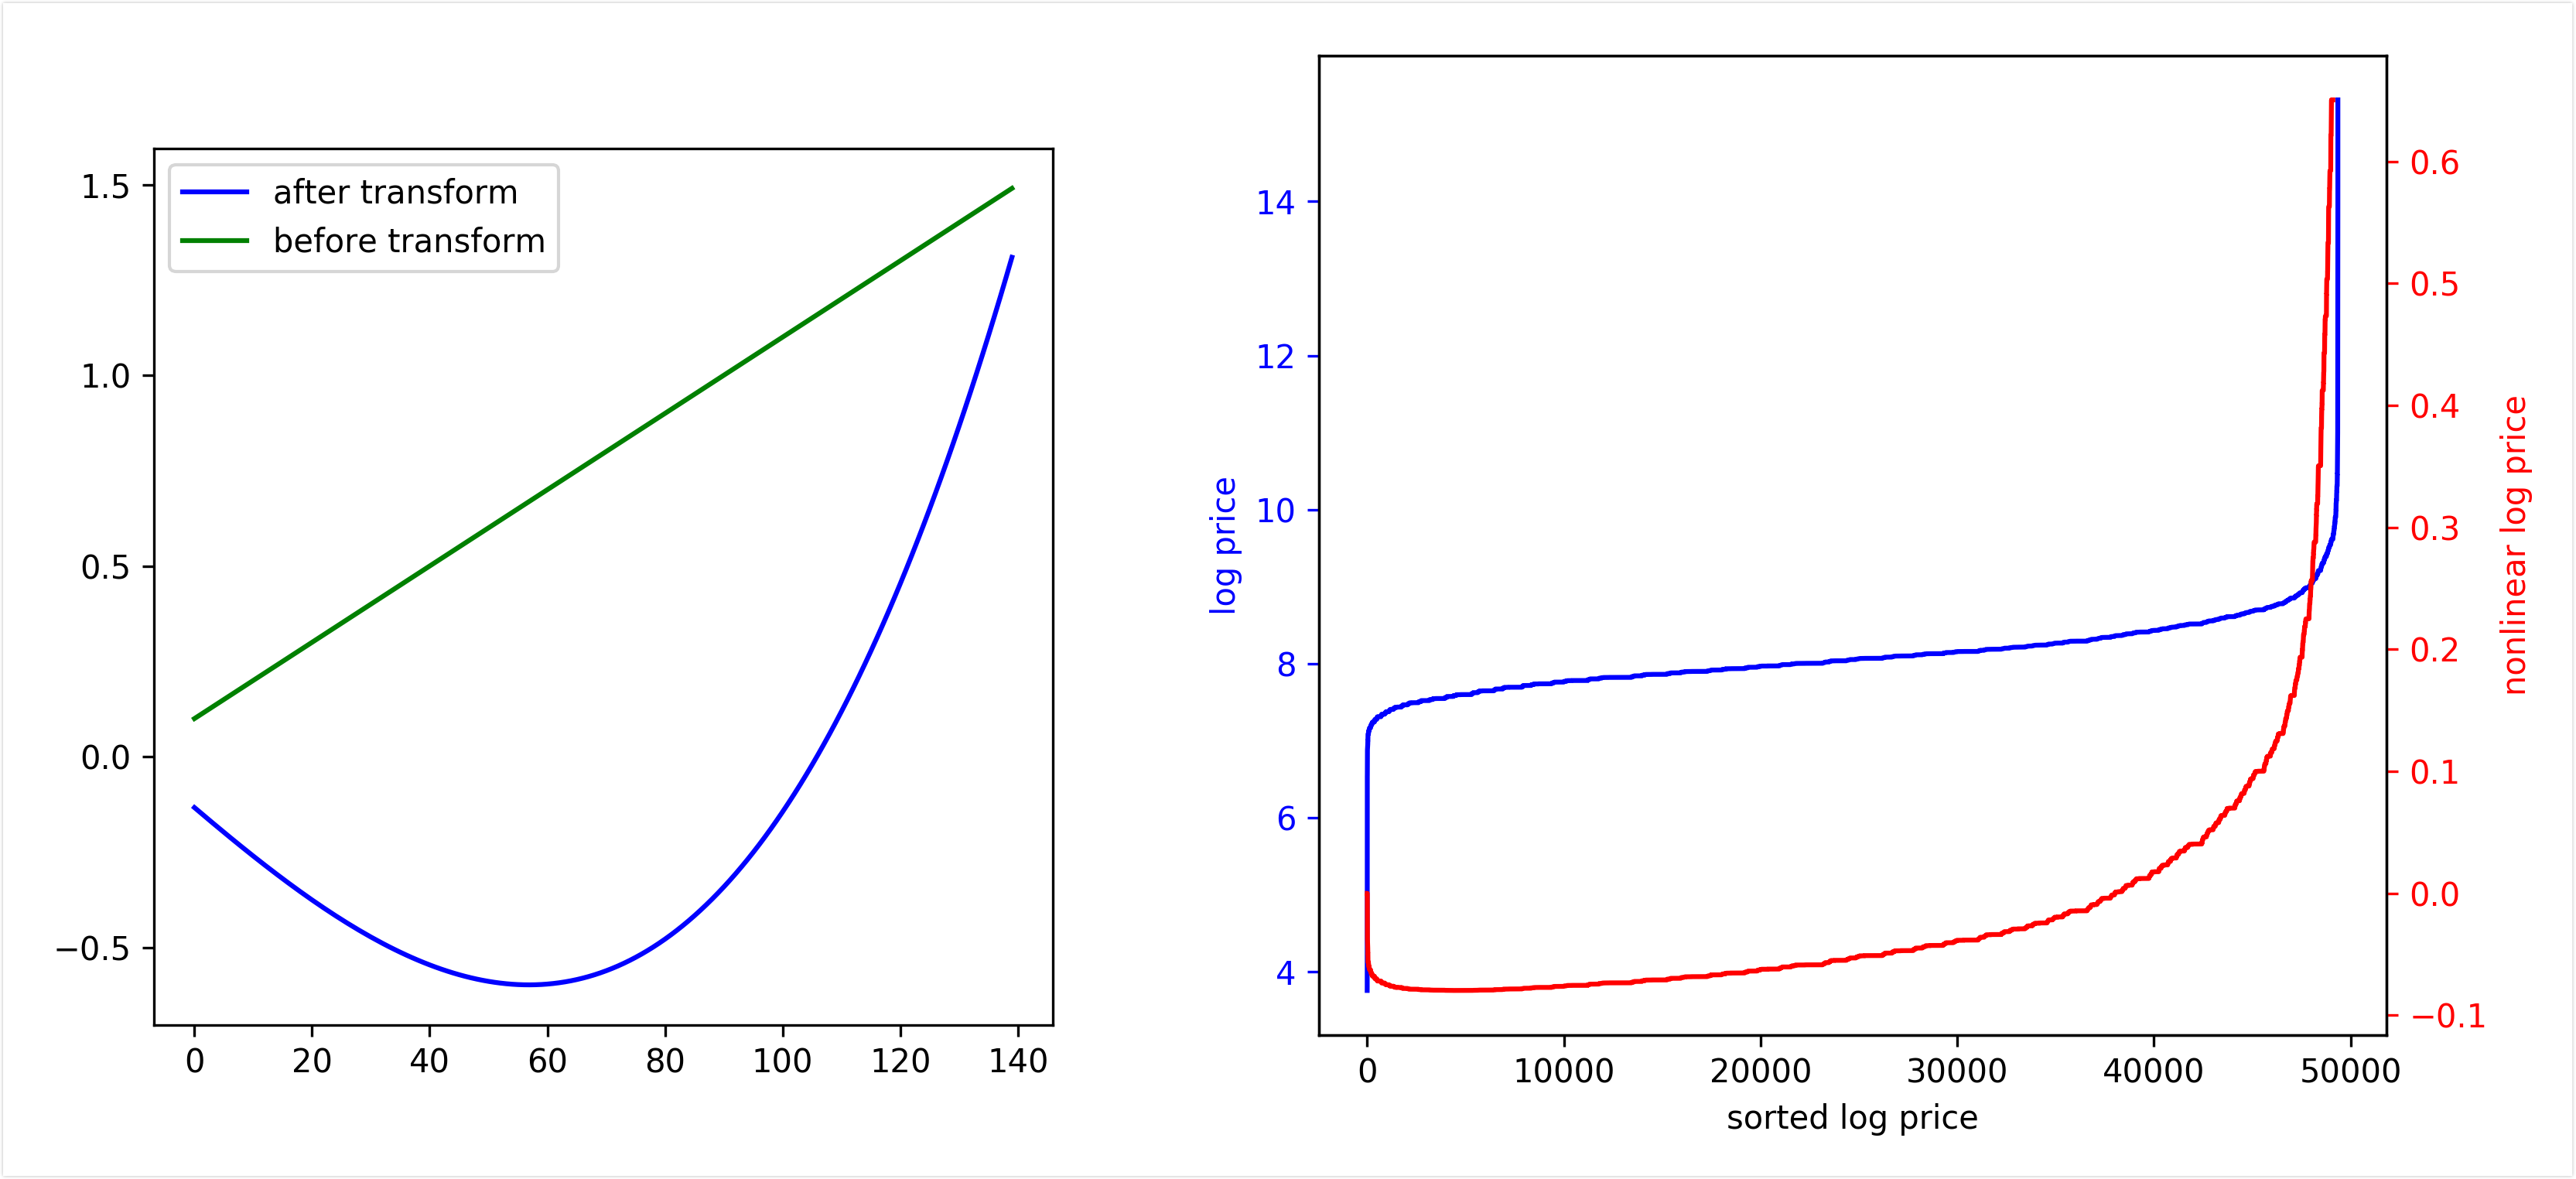
\includegraphics[width=0.85\linewidth]{images/nonlinear.png}\\}
  \vspace{0.2em}
 
\noindent\textbf{4. Human Factor - The Manager}\vspace{-0.5em}
  
  \begin{multicols}{2}
    We look at the performance of mangers, which is defined by the ratios of apartments in each interest-level, under his/her management, and an overall score of the manager is computed based on the three ratios. This set of features is an alternative to categorizing manager ID number.
    
    \noindent An overview of the manager performance:
    
    {\centering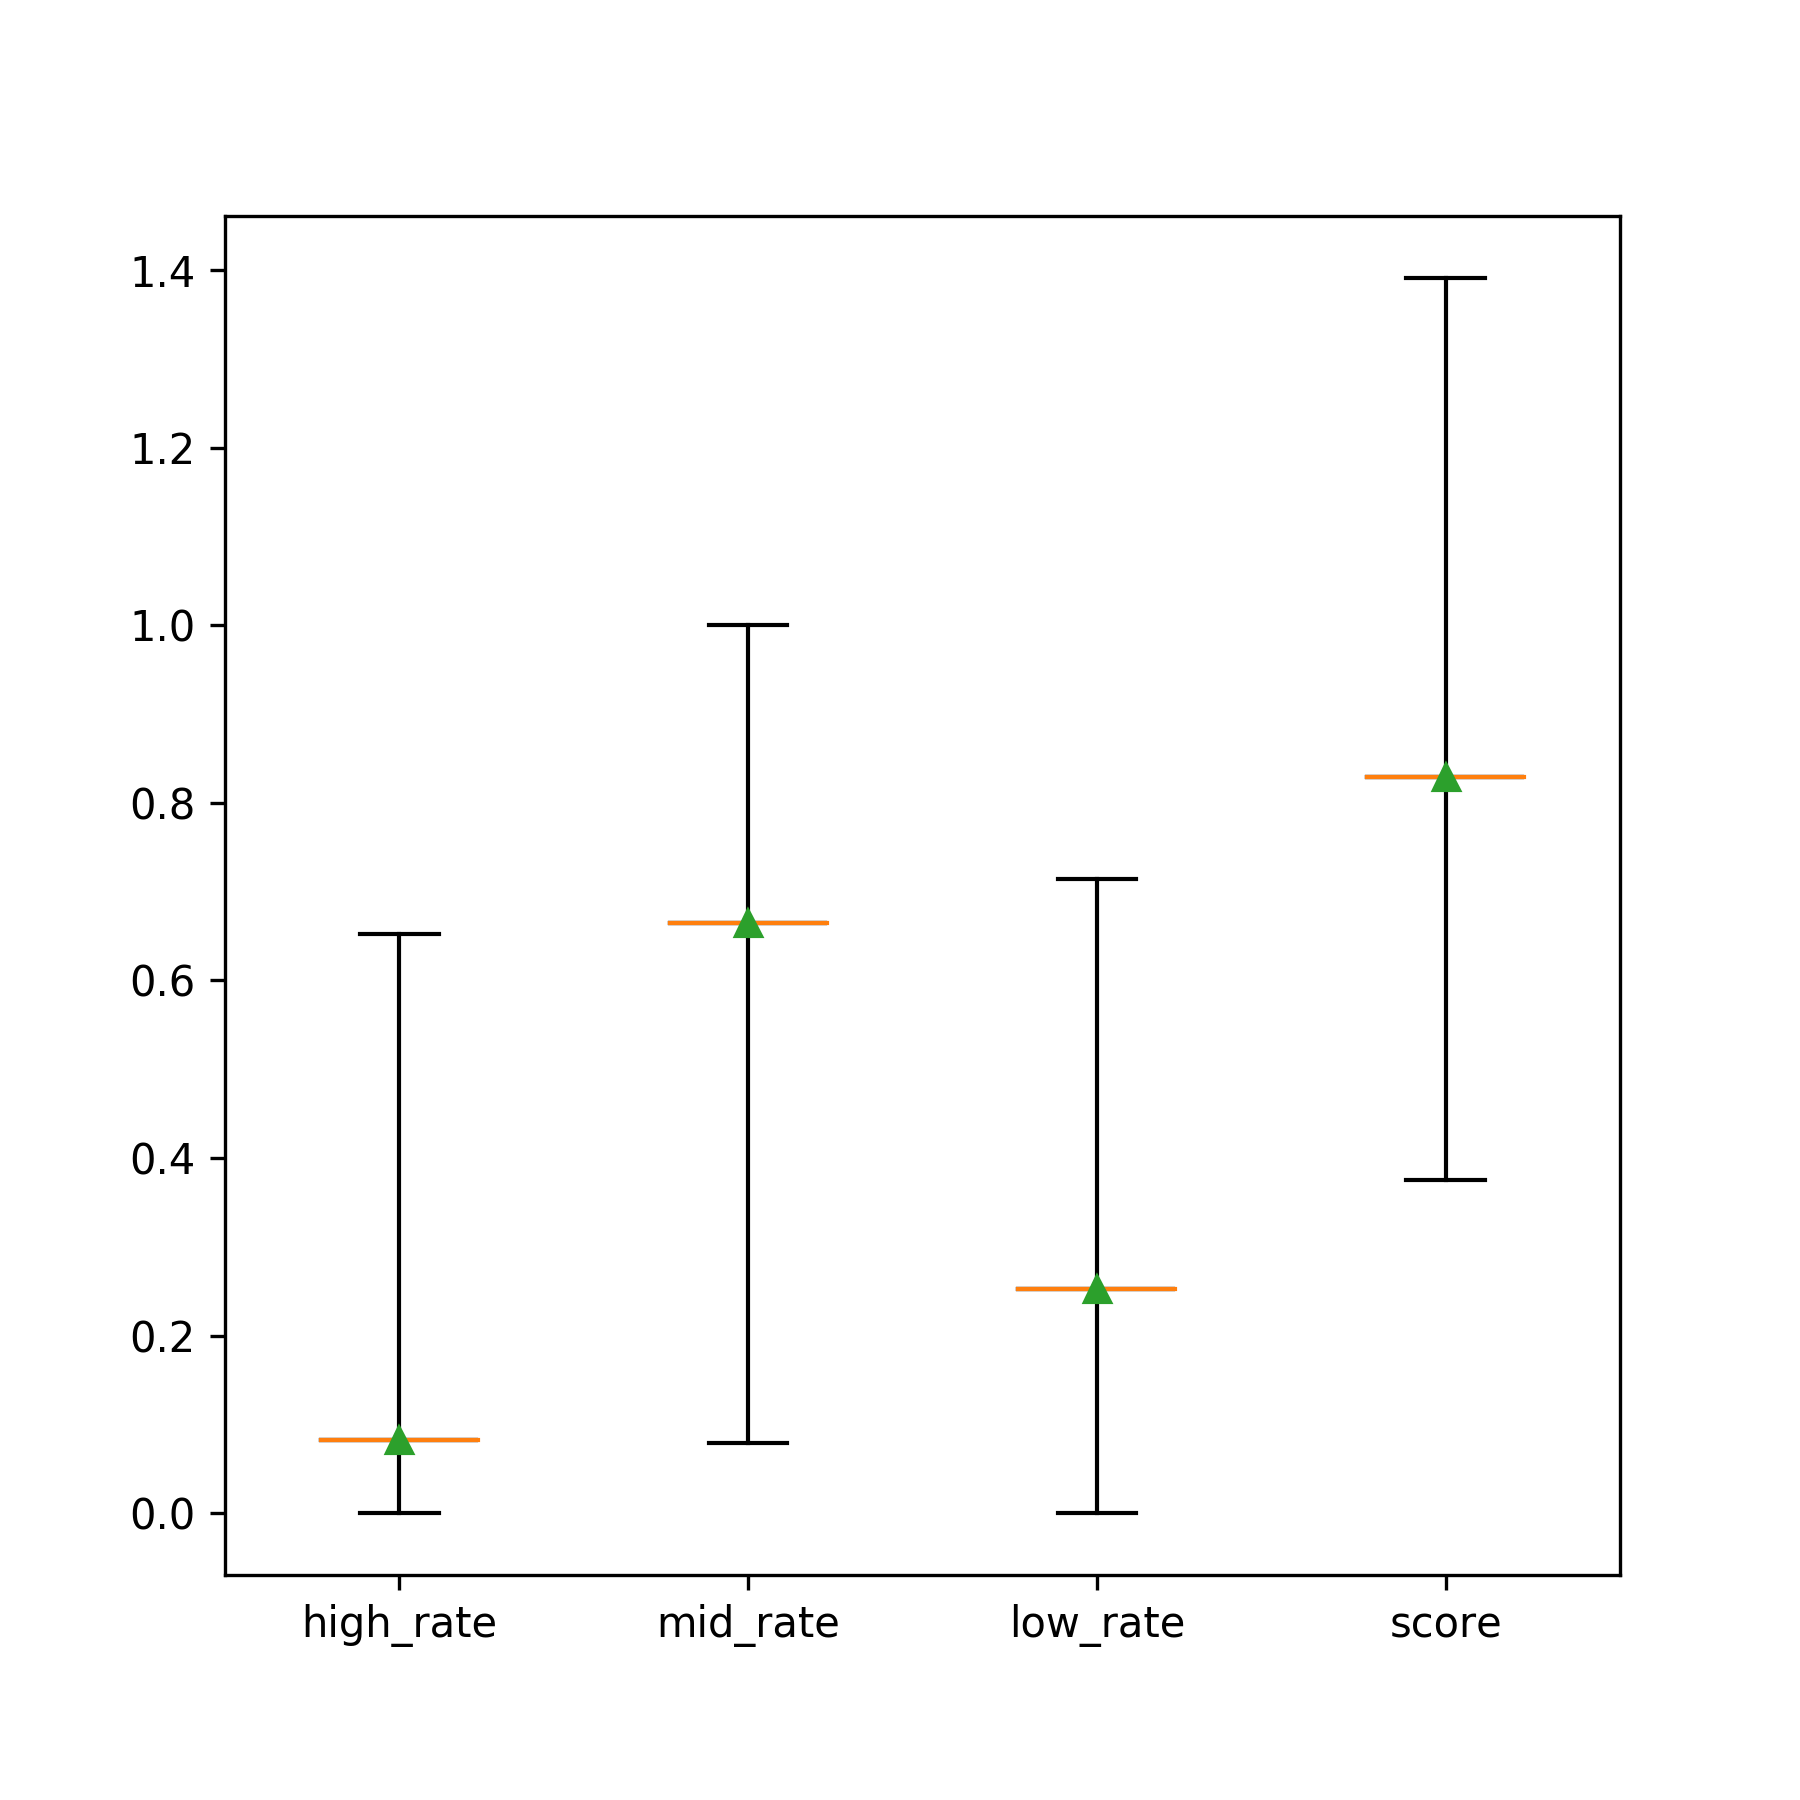
\includegraphics[width=0.95\linewidth]{images/manager_skill.png}}
    
  \end{multicols}

\noindent\textbf{5. Clustering on Geographical Data}\vspace{-0.5em}

  \begin{multicols}{2}
    With the assumption that close locations will have similar community services, convenience of transportation and so on, we will compare the price of each apartment with the median in its ``community'', which is implemented by clustering on latitude and longitude features. This gap between the price of a apartment with the median price can be regarded as a specific factor of the apartment.
    (An Example of 10 clusters)
    
    {\centering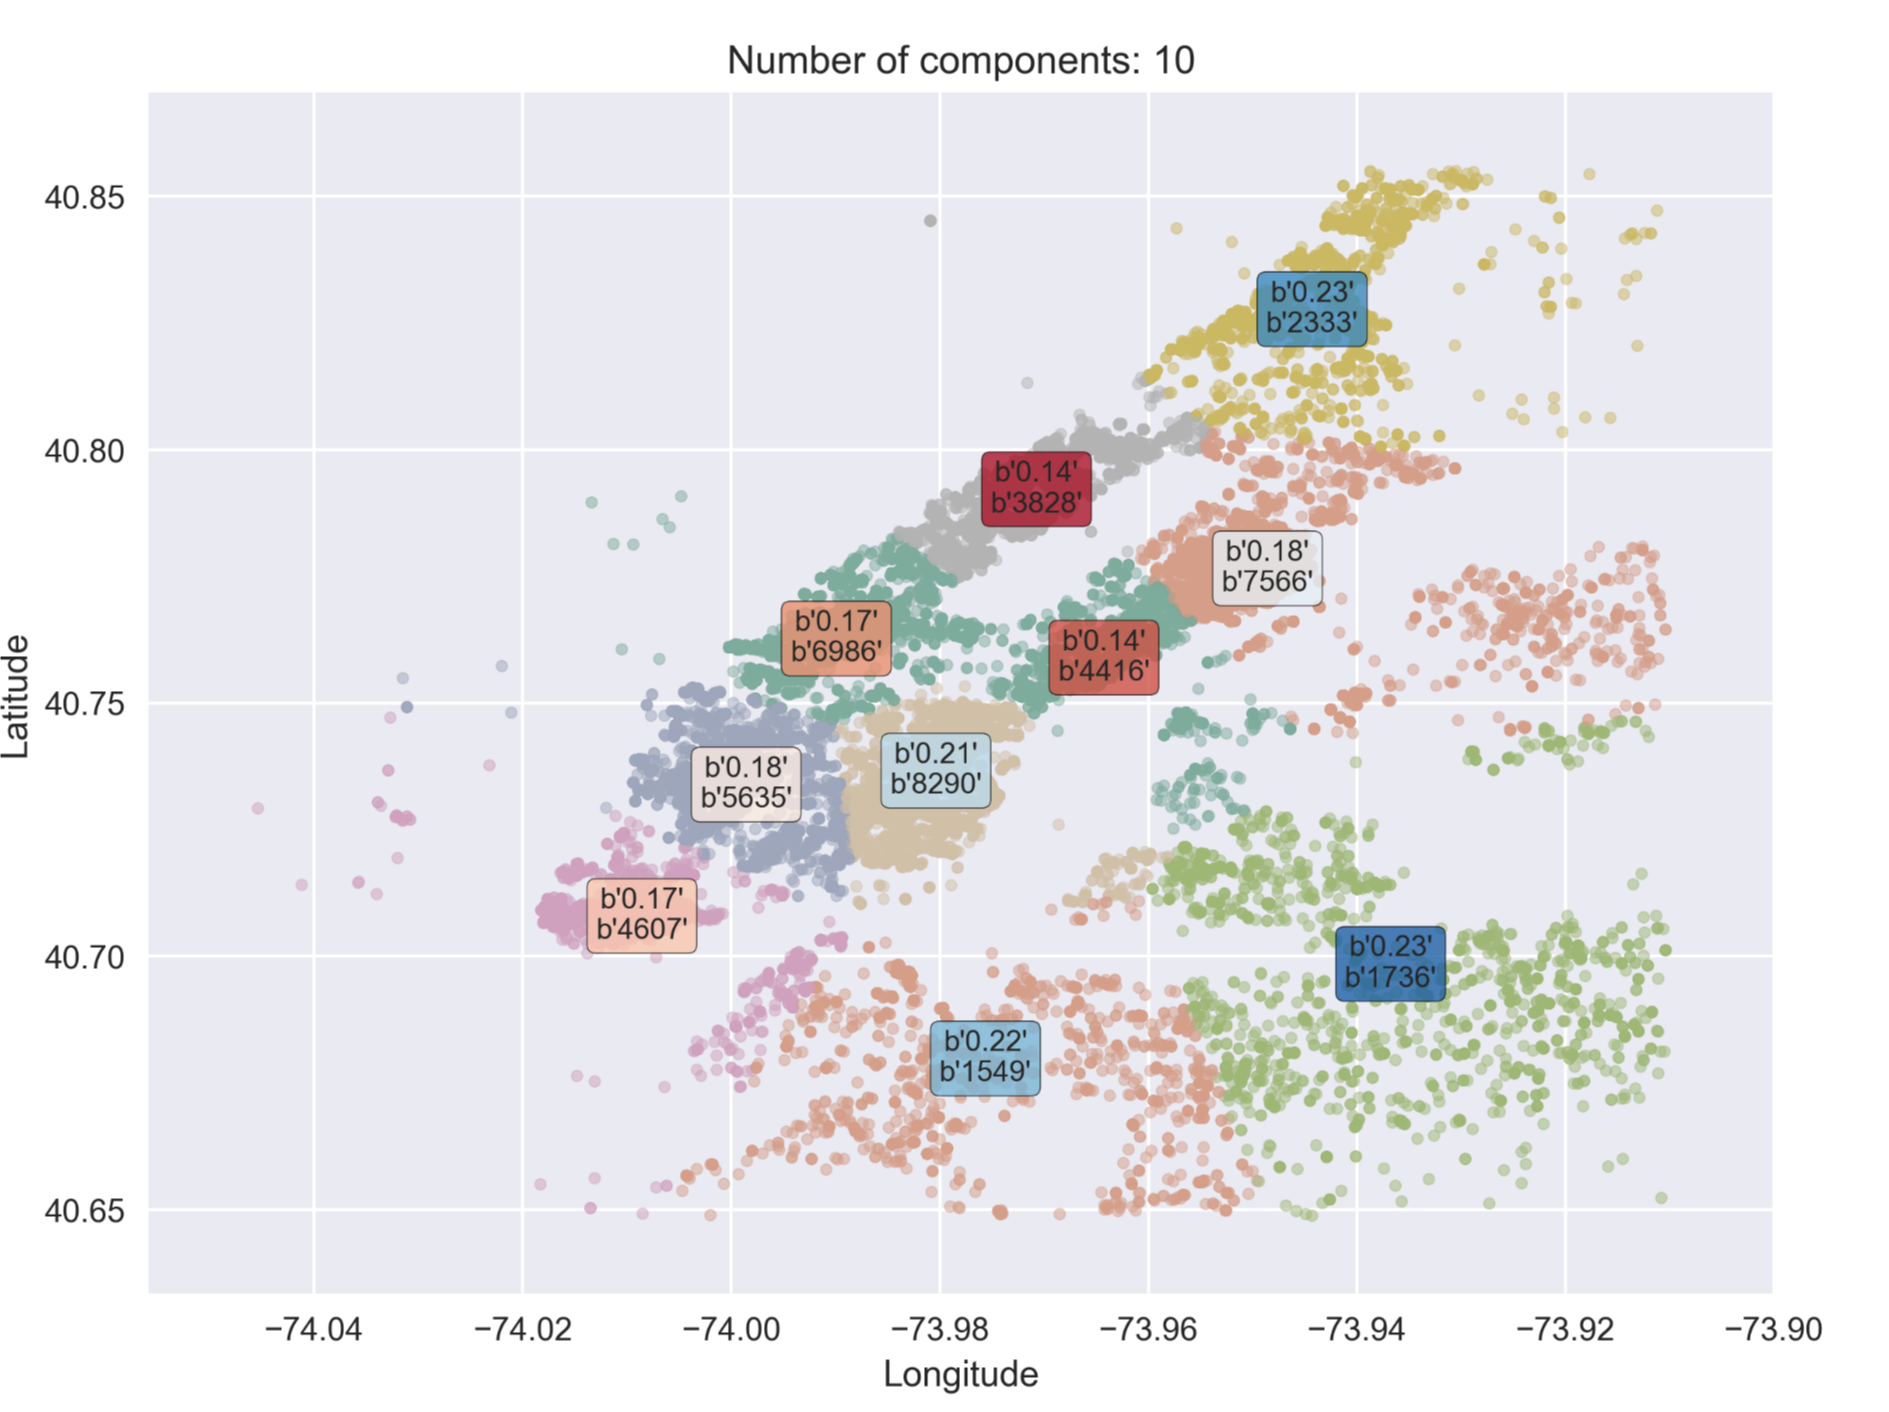
\includegraphics[width=0.99\linewidth]{images/cluster_10.png}}
  \end{multicols} 

\noindent\textbf{6. What Do Descriptions "Say"?}\vspace{0.2em}

  The first step of processing vocabular data %(``features'' and ``description'') 
  is to remove synonyms, as the descriptions in the listings are entered by different managers/officers. 
  Then, we obtain sparse features of tf-idf information through word-map vectorization. Regularization is introduced to avoid overfitting. 
  \vspace{0.2em} 
  
\end{multicols}
}

%%%%%%%%%%%%%%%%%%%%%%%%%%%%%%%%%%%%%%%%%%%%%%%%%%%%%%%%%%%%%%%%%%%%%%%%%%%%%%
\headerbox{Results}{name=result,column=3,row=0}{
  %%%%%%%%%%%%%%%%%%%%%%%%%%%%%%%%%%%%%%%%%%%%%%%%%%%%%%%%%%%%%%%%%%%%%%%%%%%%%%
  After repeated testing, we conclude that the set of features including numerical features (original and added), categorical features, non-linear price, manager scores and the tf-idf features (150-200) gives the overall best performance, with gradient boosting methods. As we adding new features into our model, boosted trees implemented with XGBoost provides with minimal error rate and highest probability of predicting the correct class.
  
  { \centering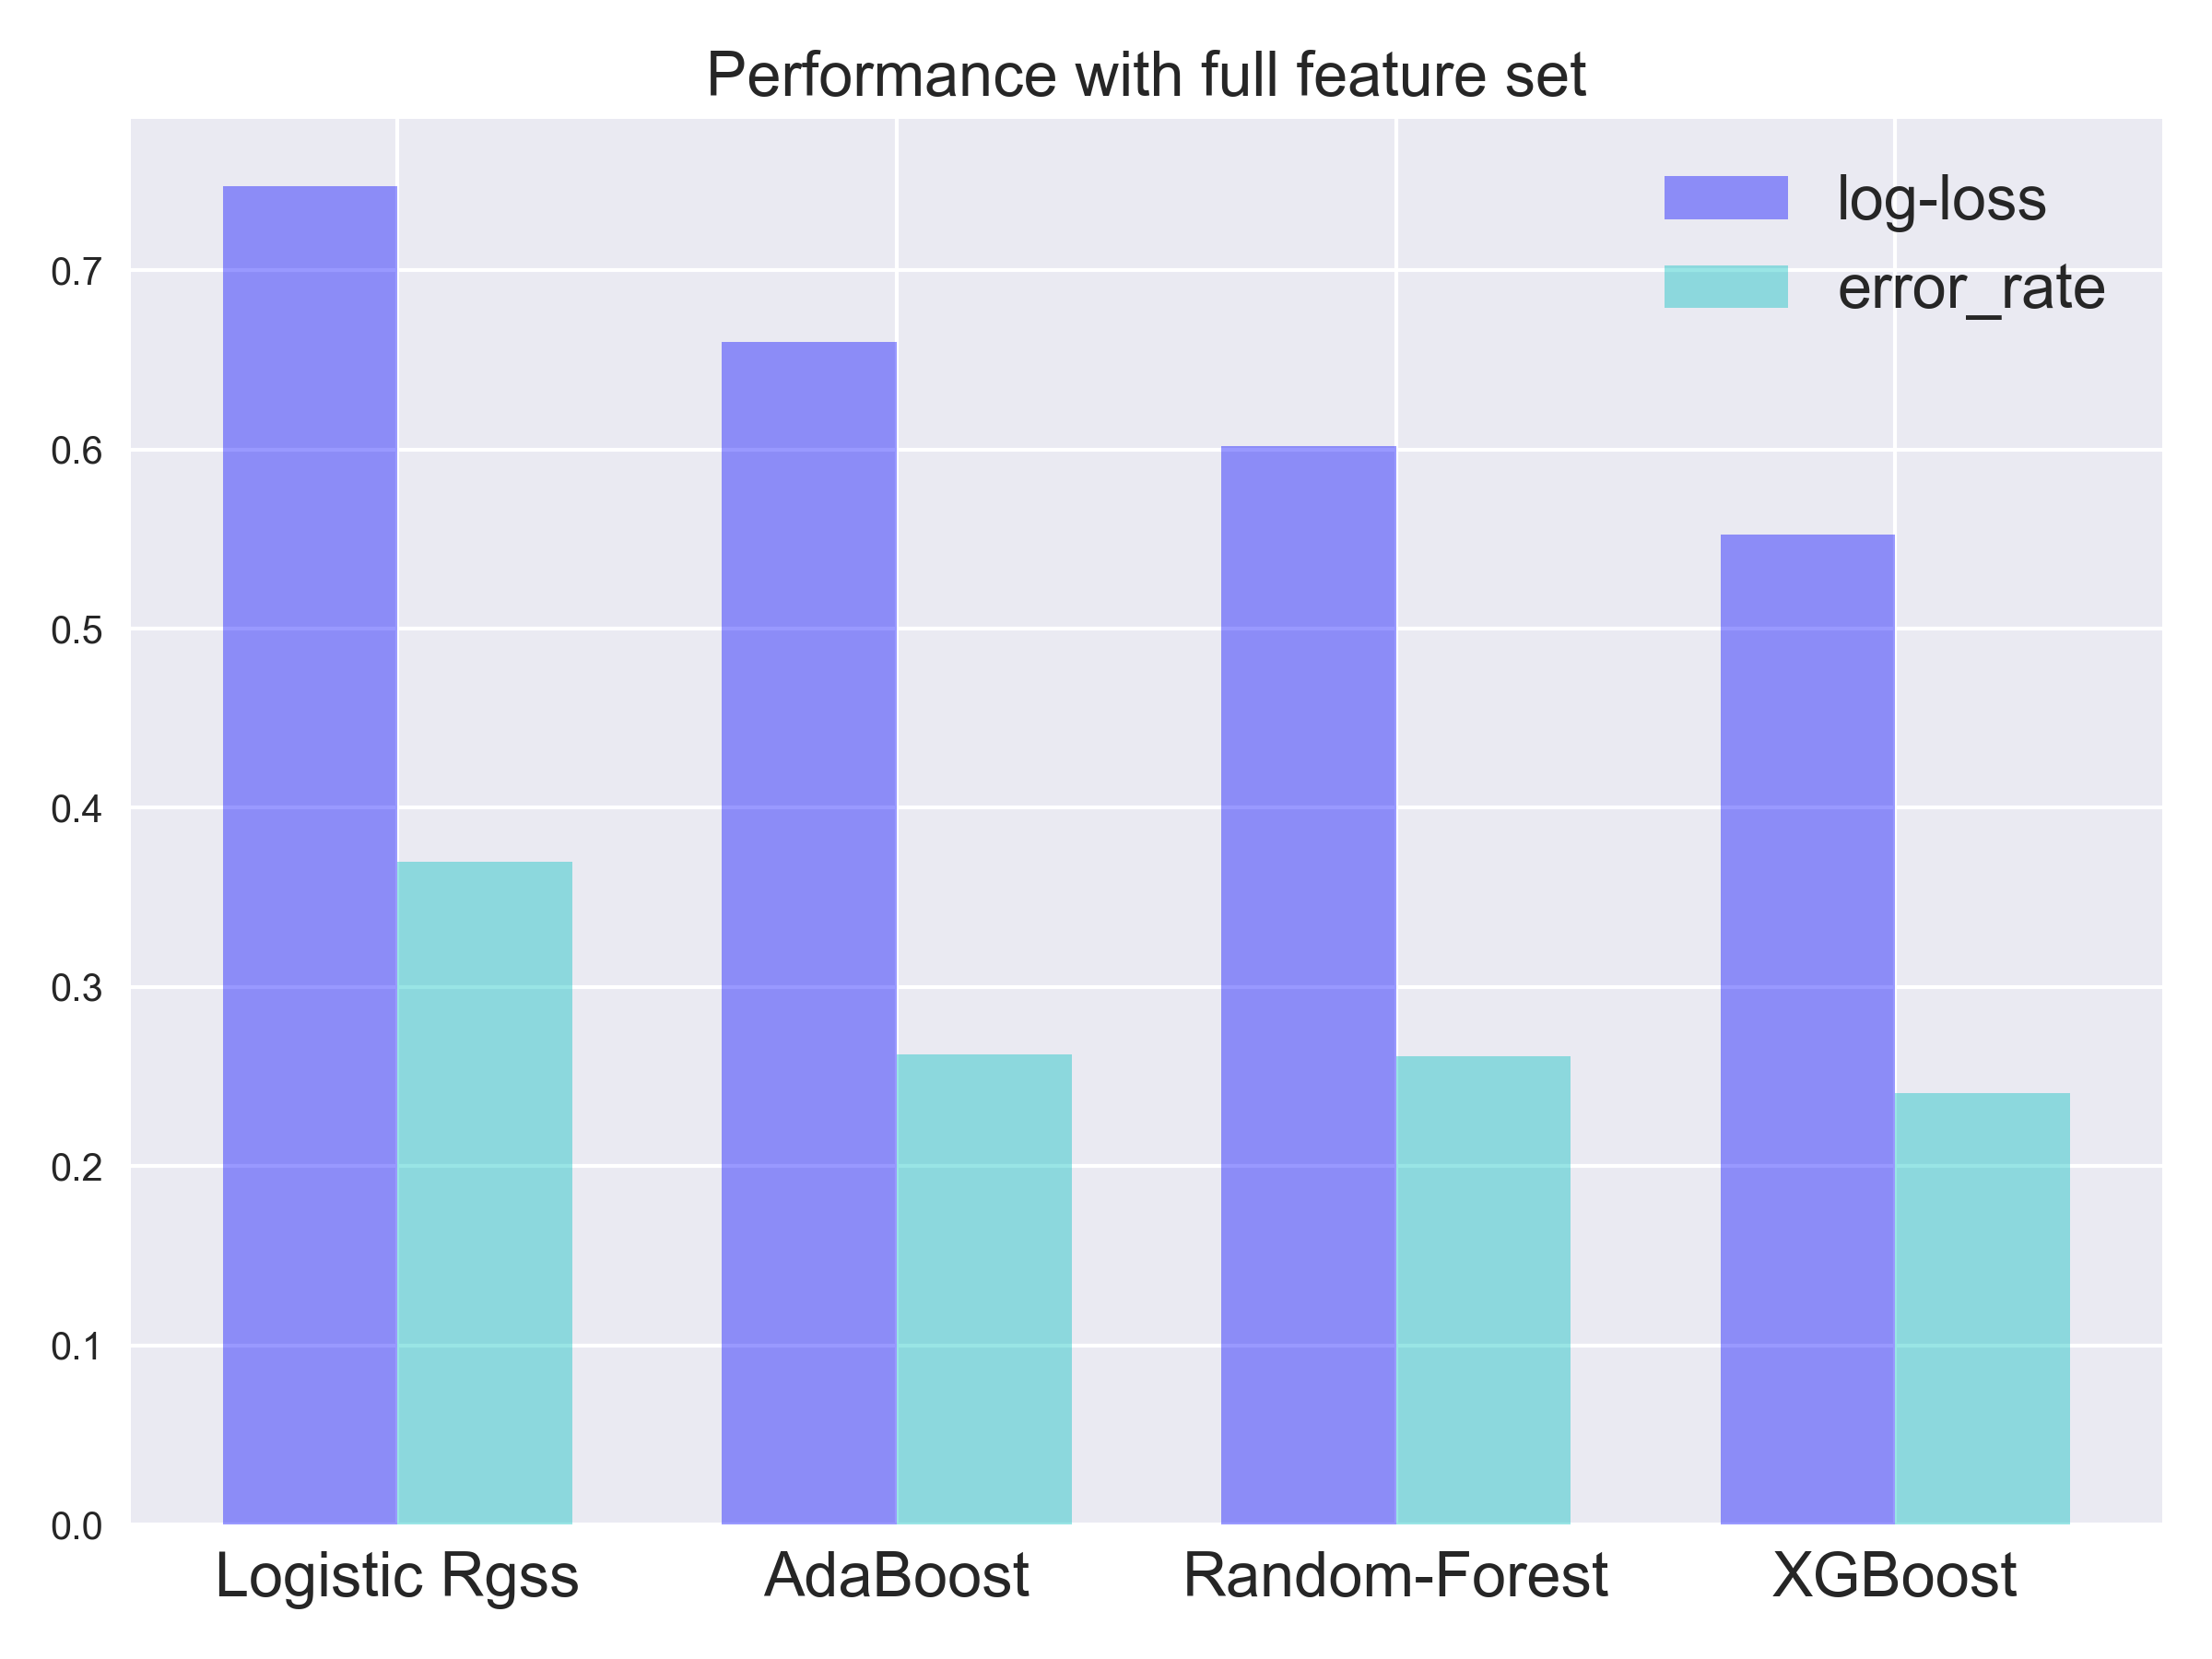
\includegraphics[width=0.95\linewidth]{images/compare_result.png}}\vspace{-0.5em}
  
  \begin{multicols}{2}
    {\footnotesize The enormous tf-idf features are not plotted in the figure of feature importance. Top vocabularies includes:\\
    \indent\textbullet ~public\_outdoor\\
    \indent\textbullet ~laundry\_in\_building\\
    \indent\textbullet ~recreation\_facilities\\
    \indent\textbullet ~eat\\
    \indent\textbullet ~24 (24/7 services)\\
    \indent\textbullet ~no\_fee\\
    \indent\textbullet ~air\_conditioning\\
    \indent\textbullet ~private\_parking\\
    \indent\textbullet ~walls\_of\_windows\\
    \indent\textbullet ~pool\\
    }
    %{\centering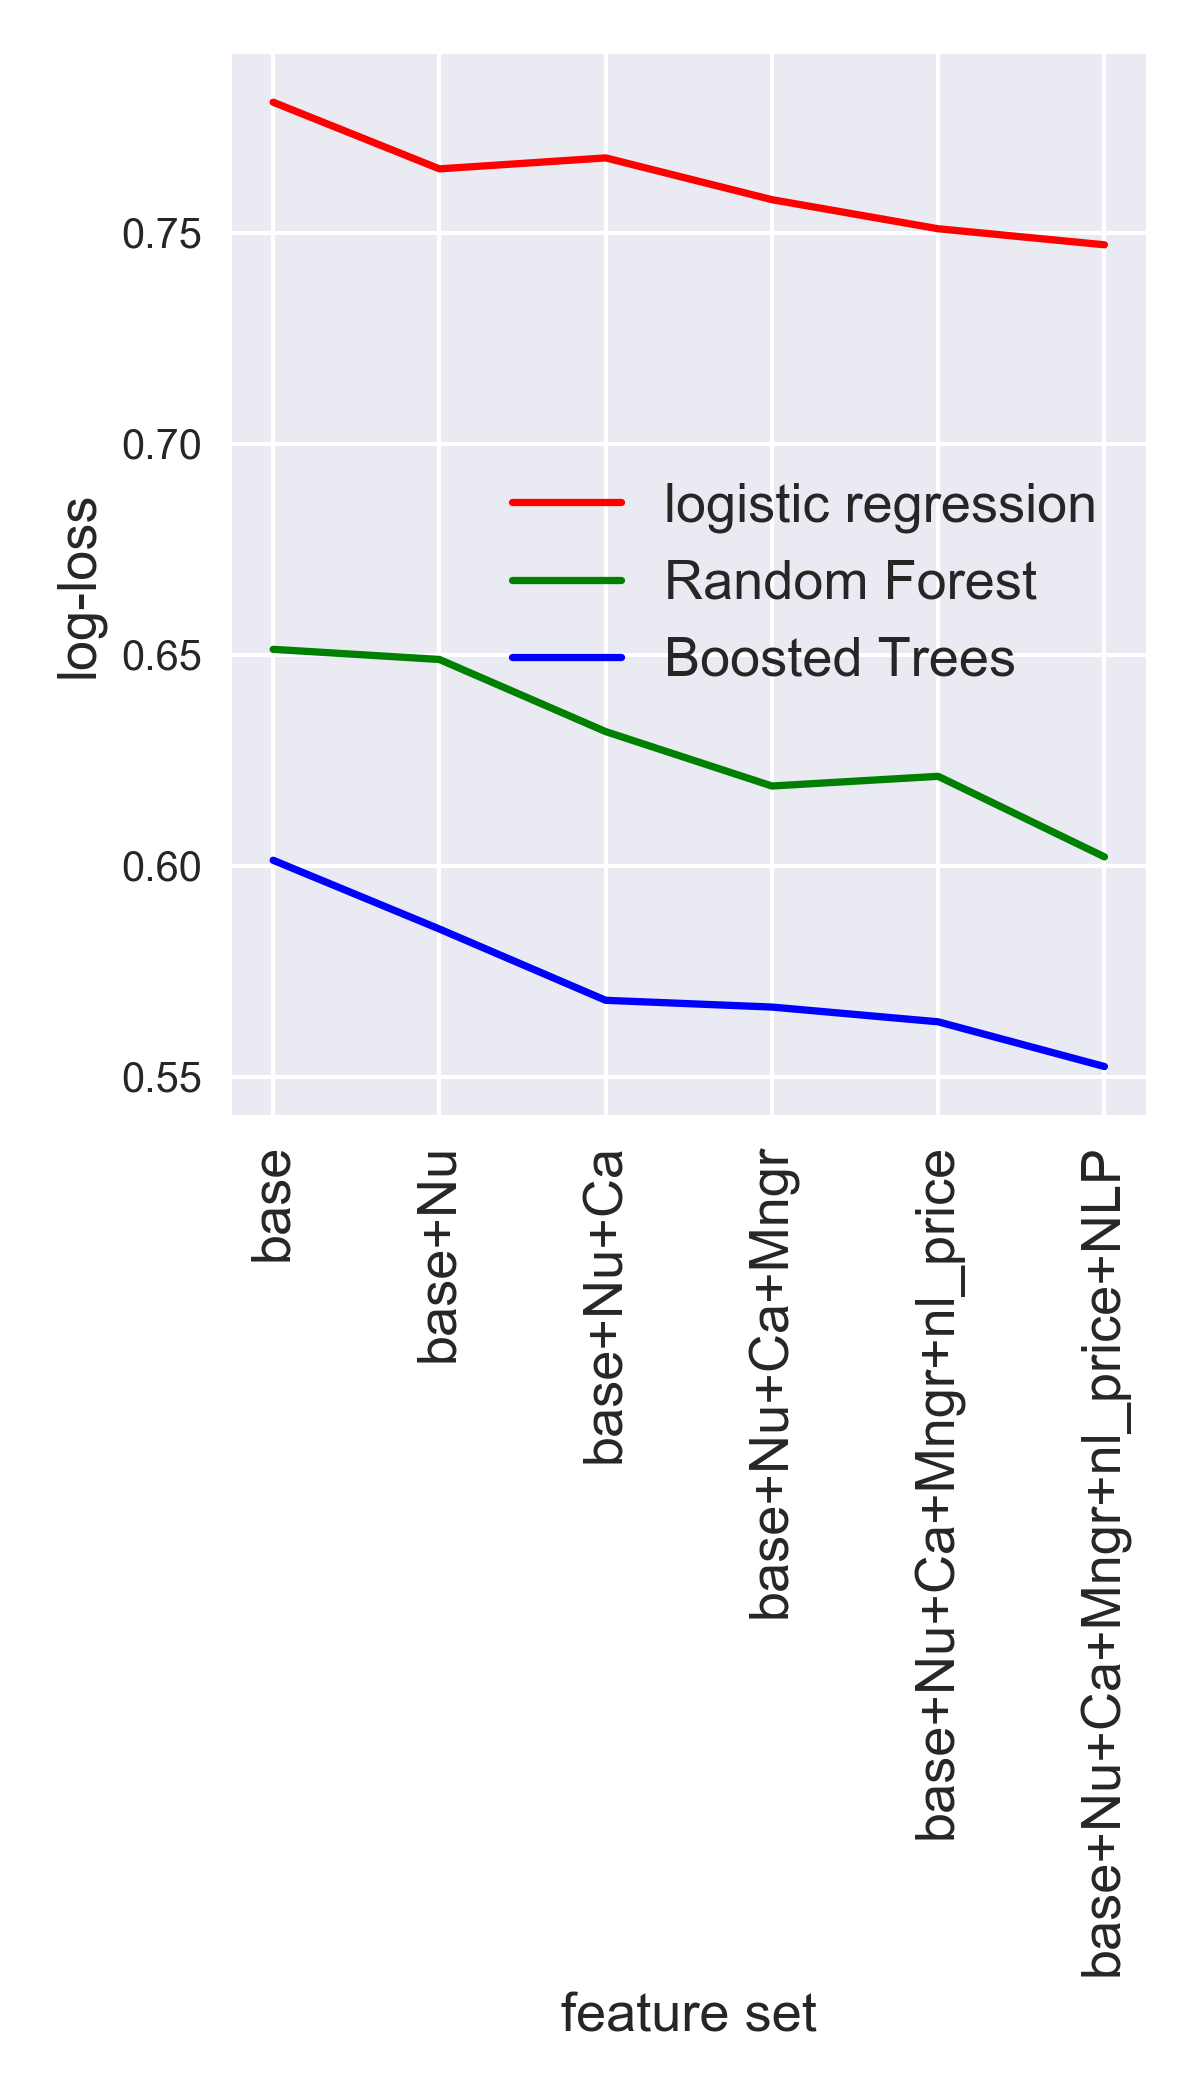
\includegraphics[width=0.99\linewidth]{images/loss_improve.png}}
    {\centering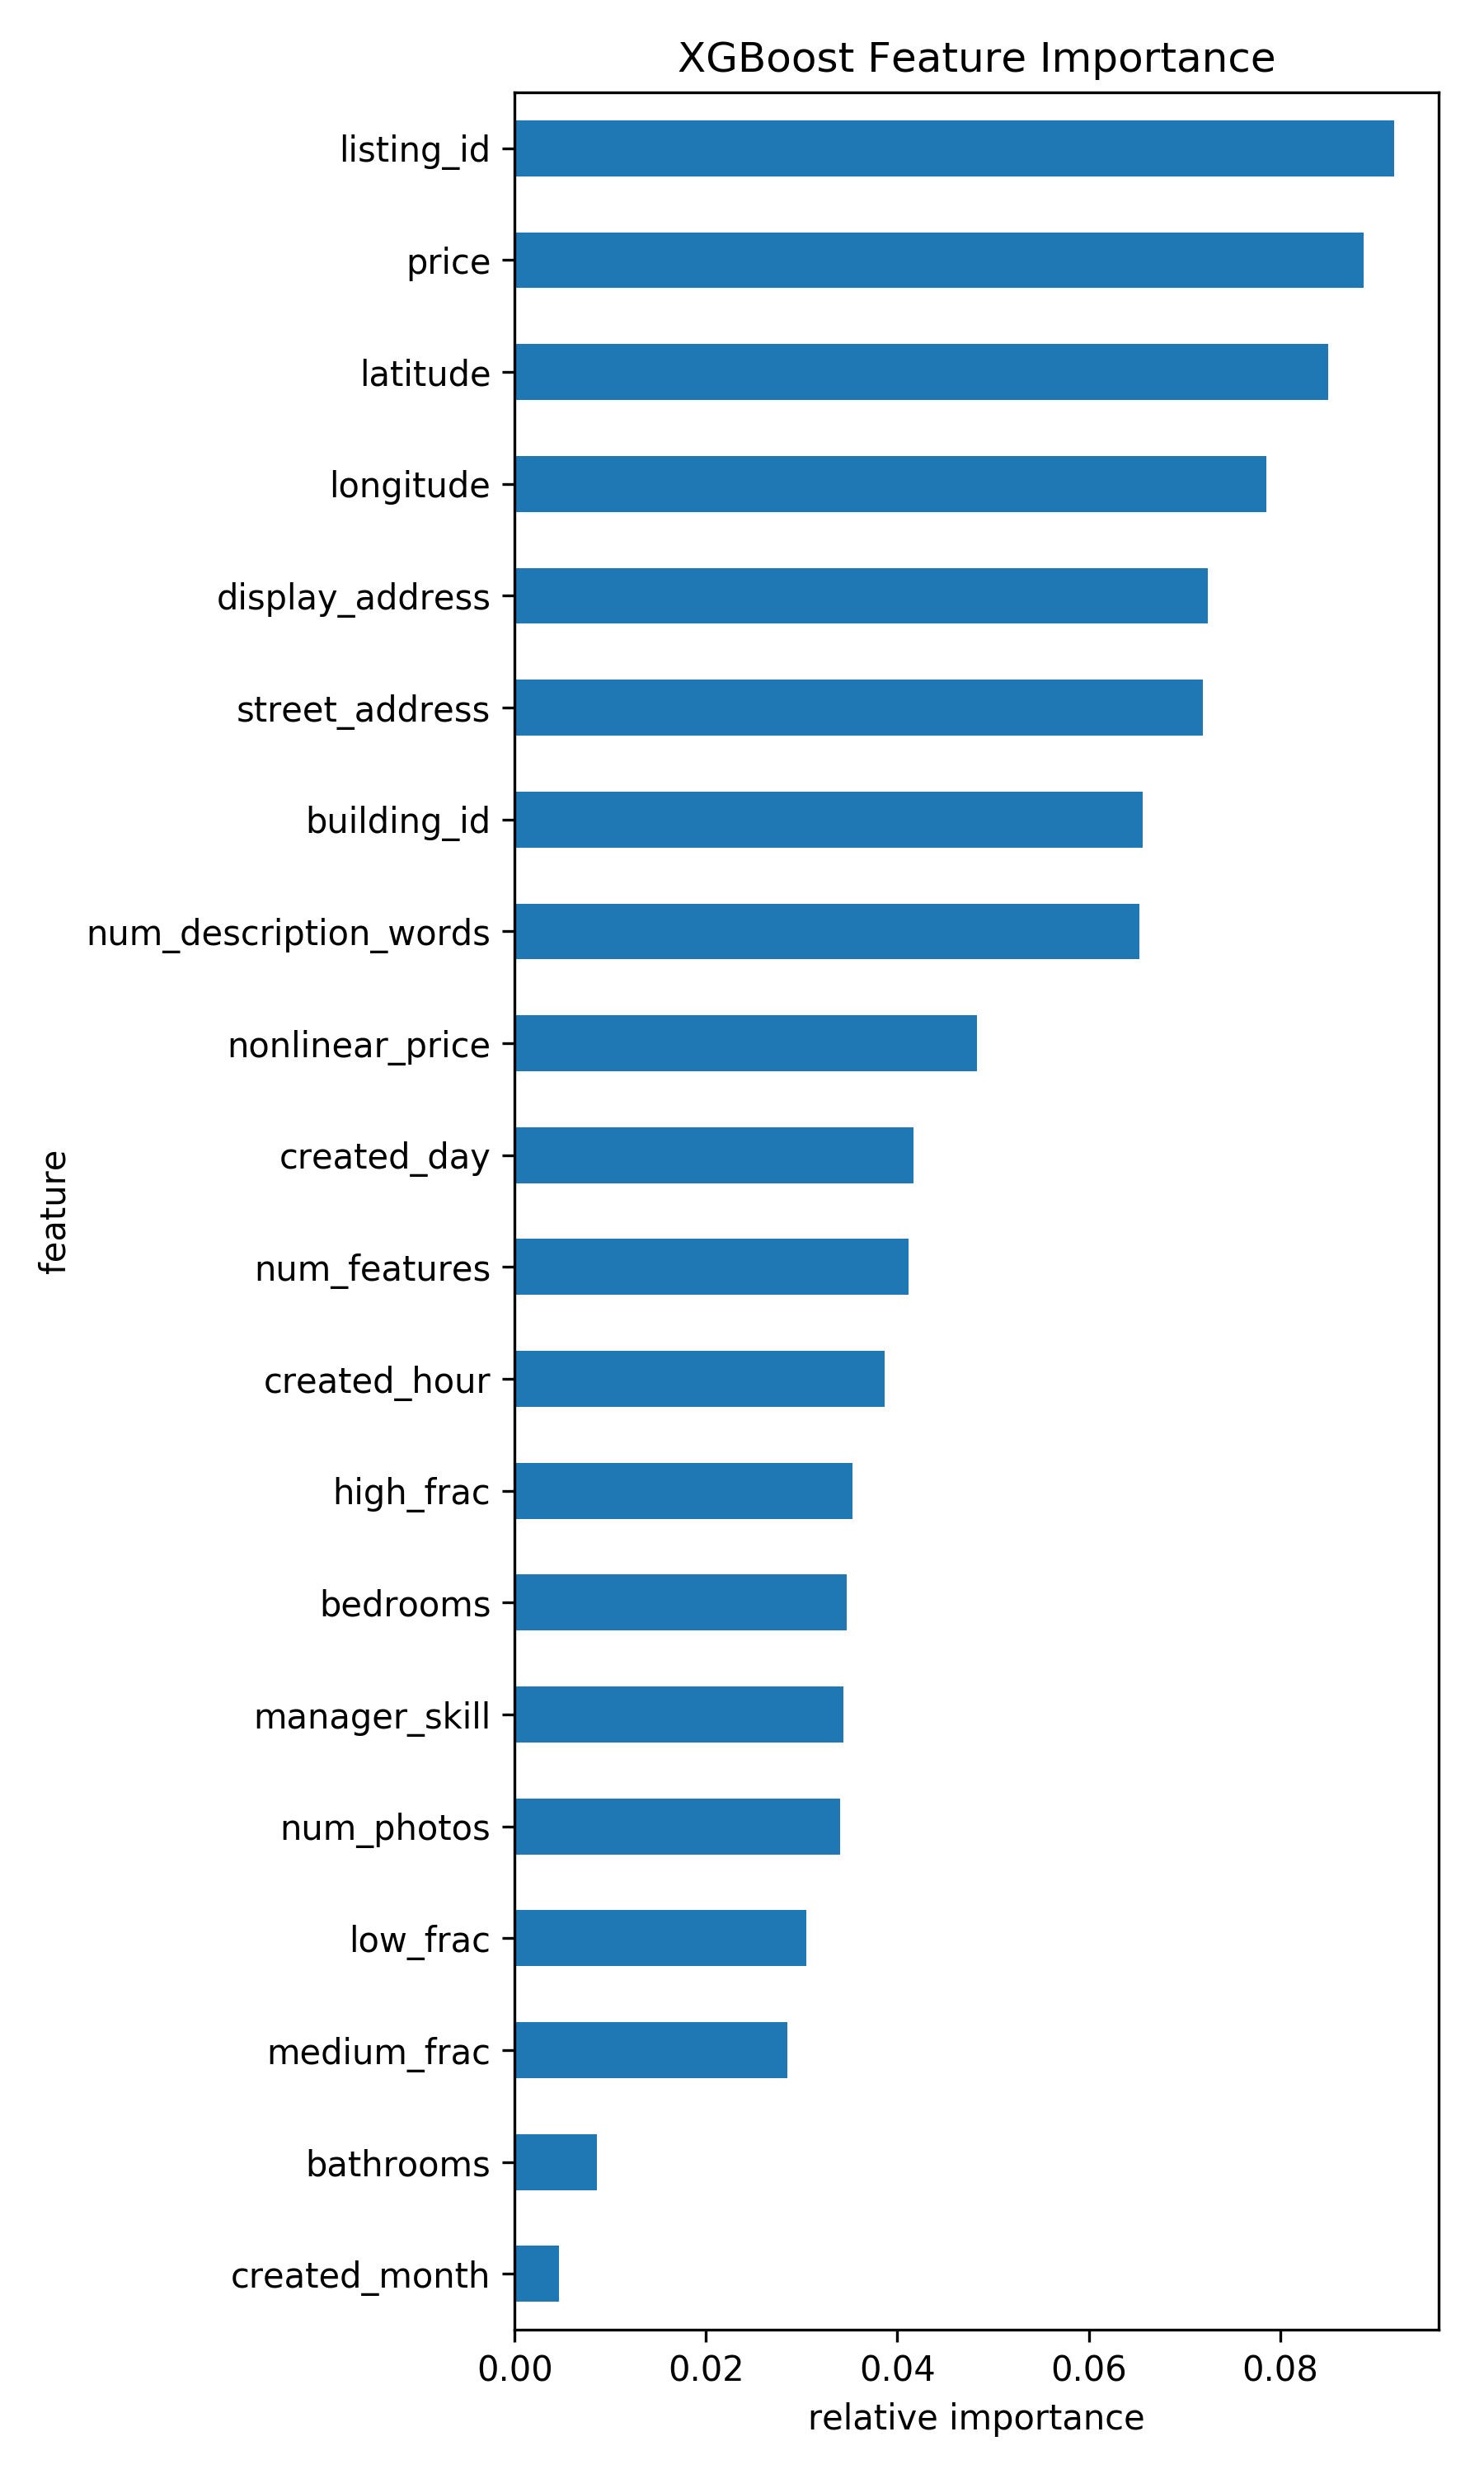
\includegraphics[width=0.99\linewidth]{images/feature_importance_xgb_1.png}}
    
  \end{multicols}
  \vspace{-0.6em}
}

%%%%%%%%%%%%%%%%%%%%%%%%%%%%%%%%%%%%%%%%%%%%%%%%%%%%%%%%%%%%%%%%%%%%%%%%%%%%%%
  \headerbox{References}
  {name=references,column=3,above=bottom}{
%%%%%%%%%%%%%%%%%%%%%%%%%%%%%%%%%%%%%%%%%%%%%%%%%%%%%%%%%%%%%%%%%%%%%%%%%%%%%%
    \smaller
    \bibliographystyle{ieee}
    \renewcommand{\section}[2]{\vskip 0.05em}
      \begin{thebibliography}{1}\itemsep=-0.01em
      \setlength{\baselineskip}{0.4em}
      \bibitem{a}
        Niculescu-Mizil, A., Caruana, R.
        \newblock Obtaining Calibrated Probabilities from Boosting
        \newblock In {\em UAI '05}
      \bibitem{b}
        Niculescu-Mizil, A., Caruana, R.
        \newblock Predicting good probabilities with supervised learning
        \newblock In {\em ICML '05}
      \bibitem{c}
        Will McGinnis.
        \newblock Beyond One-Hot: Aa Exploration of Categorical Variables.
        \newblock In {\em Will's Noise}
      \end{thebibliography}
   \vspace{0.3em}
}

%%%%%%%%%%%%%%%%%%%%%%%%%%%%%%%%%%%%%%%%%%%%%%%%%%%%%%%%%%%%%%%%%%%%%%%%%%%%%%
  \headerbox{Future Steps}
  {name=next_step,column=1,span=2,aligned=references, above=bottom}{
%%%%%%%%%%%%%%%%%%%%%%%%%%%%%%%%%%%%%%%%%%%%%%%%%%%%%%%%%%%%%%%%%%%%%%%%%%%%%%
  \begin{multicols}{2}
    There are room photos on the website for most of the listings, which provides additional high dimensional data. Neural Networks will be a good candidate to learn from the image features.
    
    Information about the convenience of transportation is missing in this dataset, though partly revealed in the descriptions. A combination with urban transportation system and medical systems (i.e. distance to the nearest train station or clinic) might be good to help. 
    
  \end{multicols}
   \vspace{0.3em}
  }
\end{poster}

\end{document}
